\chapter{Design and Methodology}
\label{chap:methodology}

\section{End-to-End System Architecture}
The proposed system architecture consists of five tightly integrated stages: physical-layer CSI capture on the ESP32 microcontroller, USB serial packet decoding, dynamic Top-$K$ subcarrier sensitivity selection, single-pass Welford online variance calculation, and digital IIR bandpass respiration extraction. Fig.~\ref{fig:overall_arch} illustrates the complete end-to-end processing pipeline.

\begin{figure}[ht]
\centering
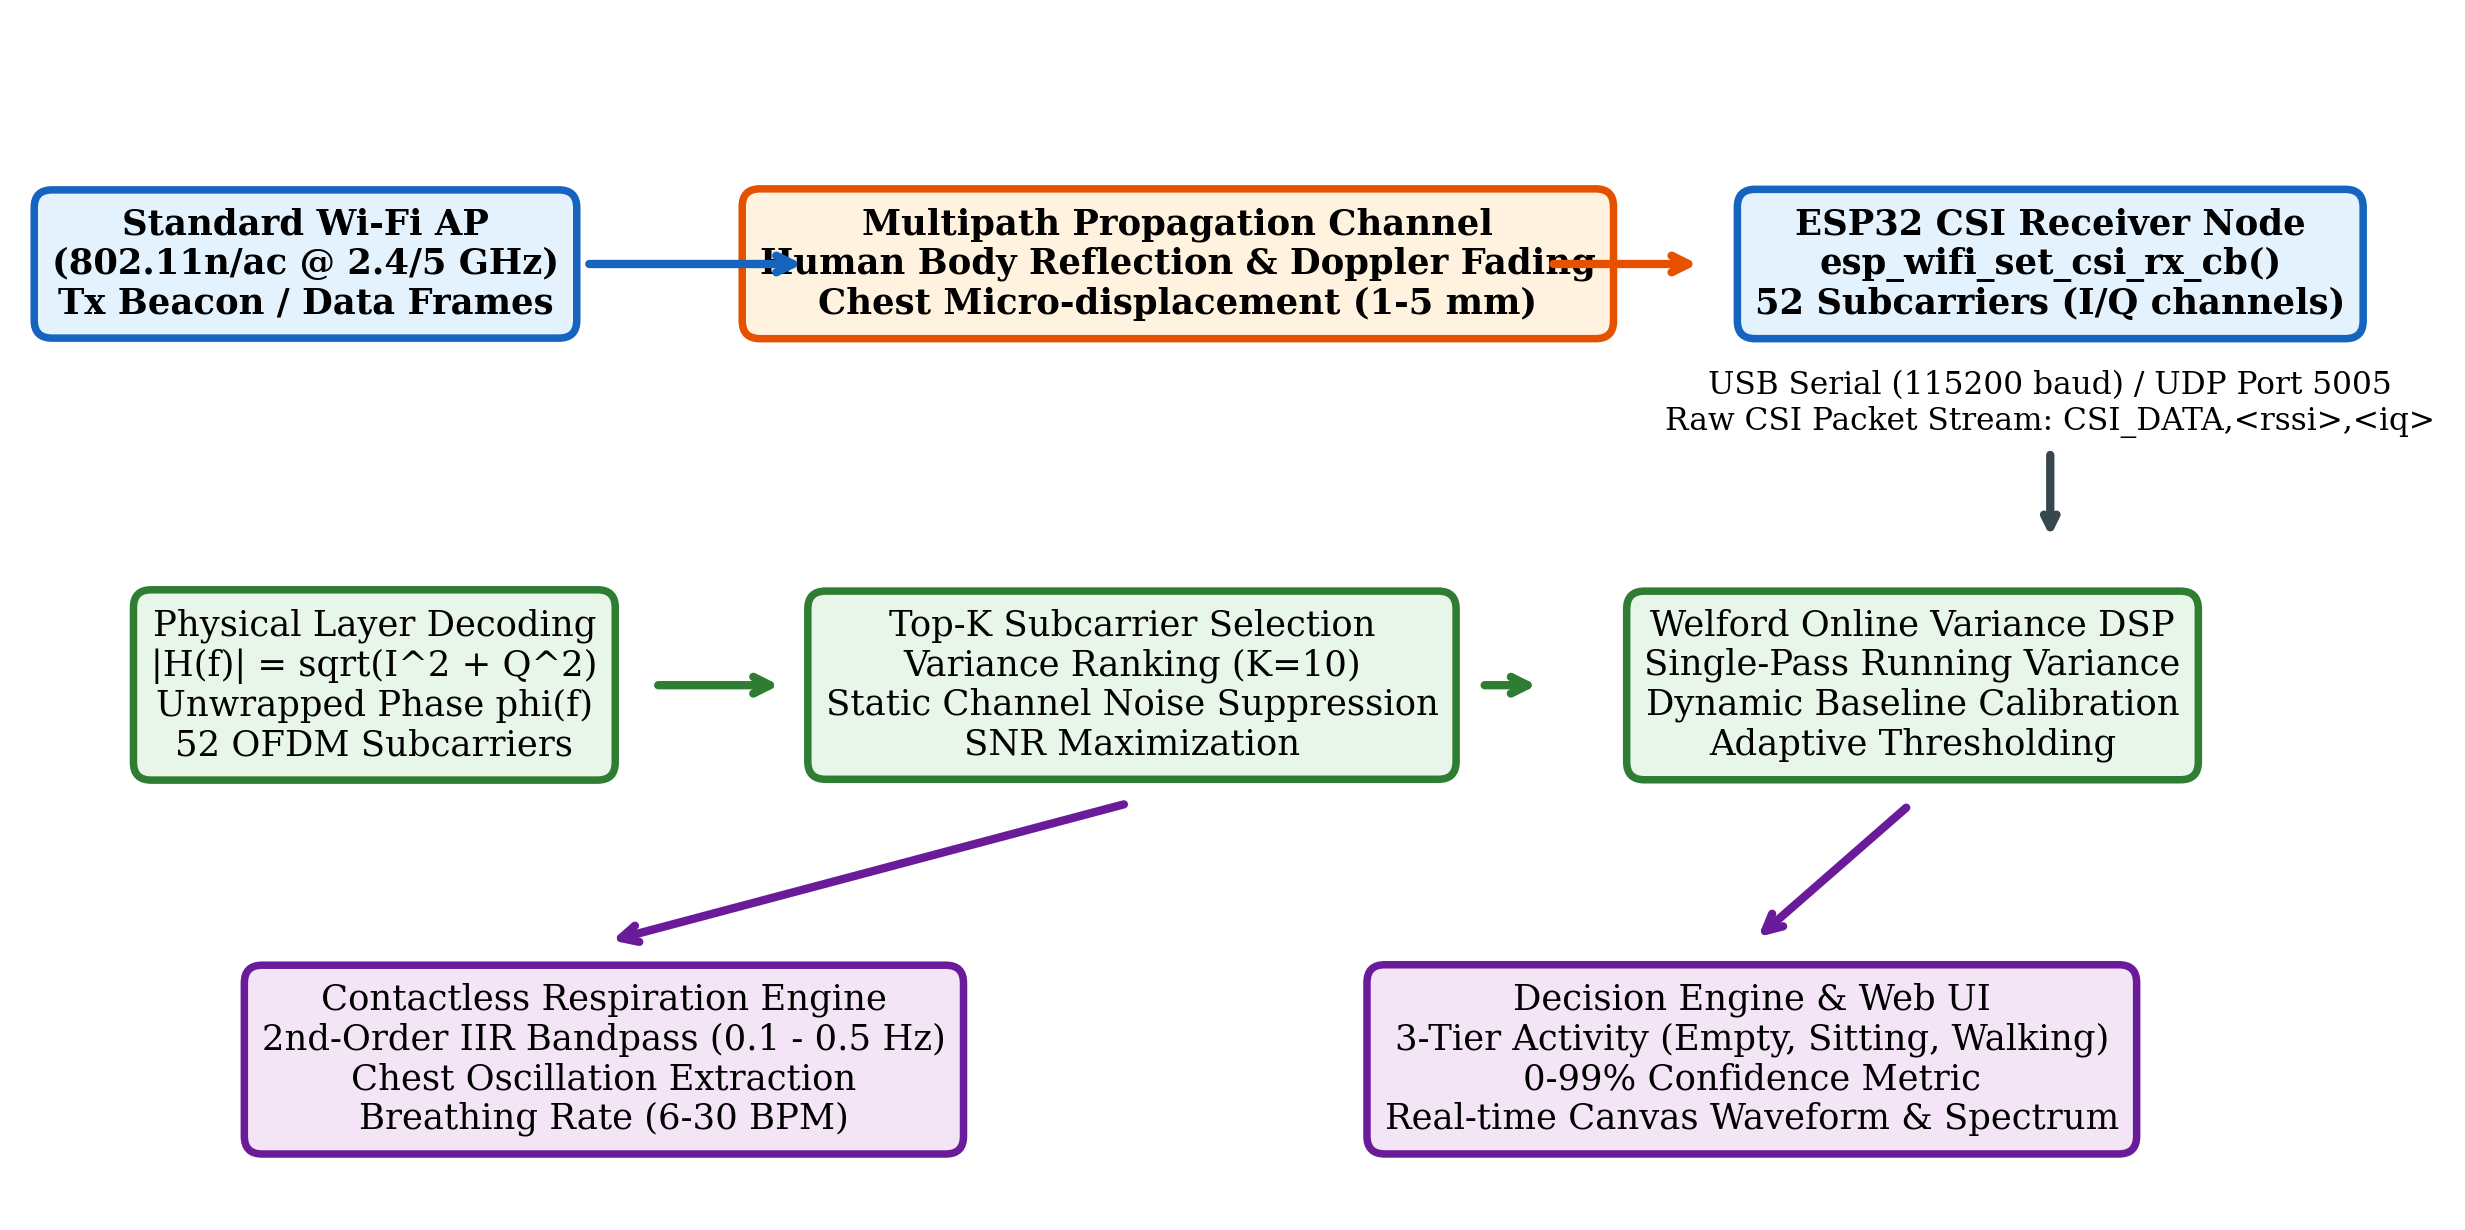
\includegraphics[width=0.95\textwidth]{figures/fig1_overall_architecture.png}
\caption{Overall architectural pipeline of the proposed commodity Wi-Fi CSI sensing system, illustrating hardware acquisition, physical-layer decoding, Top-$K$ subcarrier filtering, Welford online variance DSP, and real-time dashboard telemetry.}
\label{fig:overall_arch}
\end{figure}

\section{Physical-Layer Wi-Fi CSI Mathematical Formulation}
In an indoor wireless environment, transmitted RF signals propagate along multiple distinct paths before reaching the receiver antenna. Under the multipath propagation model, the received signal $Y(f, t)$ at frequency $f$ and time $t$ is expressed as:
\begin{equation}
Y(f, t) = X(f, t) \cdot H(f, t) + W(f, t)
\label{eq:channel_model}
\end{equation}
where $X(f, t)$ is the transmitted signal, $W(f, t)$ denotes additive white Gaussian noise (AWGN), and $H(f, t)$ is the complex Channel Frequency Response (CFR):
\begin{equation}
H(f, t) = \sum_{l=1}^L \alpha_l(t) e^{-j 2\pi f \tau_l(t)}
\label{eq:cfr_sum}
\end{equation}
Here, $L$ represents the total number of multipath trajectories, while $\alpha_l(t)$ and $\tau_l(t)$ denote the time-varying attenuation factor and propagation delay along the $l$-th path, respectively.

When a human body is present within the Fresnel zone between transmitter and receiver, the multipath channel partitions into static and dynamic components:
\begin{equation}
H(f, t) = H_{static}(f) + H_{dynamic}(f, t)
\label{eq:cfr_split}
\end{equation}
where $H_{static}(f) = \sum_{l \in L_s} \alpha_l e^{-j 2\pi f \tau_l}$ accounts for direct line-of-sight propagation and reflections from stationary walls and furniture, while $H_{dynamic}(f, t) = \sum_{m \in L_d} \alpha_m(t) e^{-j 2\pi f \tau_m(t)}$ encapsulates reflections from the moving human body and oscillating thoracic wall.

The ESP32 physical-layer baseband delivers CSI as discrete In-phase ($I$) and Quadrature ($Q$) signed integer components for each subcarrier index $k \in \{1, 2, \dots, 52\}$ in 20~MHz 802.11n channels:
\begin{equation}
H_k = I_k + j Q_k
\label{eq:iq_decomp}
\end{equation}
The instantaneous subcarrier amplitude $|H_k|$ and raw phase $\theta_k$ are derived via:
\begin{align}
|H_k| &= \sqrt{I_k^2 + Q_k^2} \label{eq:amp} \\
\theta_k &= \arctan\left(\frac{Q_k}{I_k}\right) \label{eq:phase}
\end{align}

\section{Subcarrier Spectrum Behavior Under Activity}
Fig.~\ref{fig:subcarrier_spectrum} illustrates the empirical subcarrier amplitude responses $|H(f)|$ across all 52 OFDM subcarriers under three distinct physical scenarios: an empty room, a human sitting and quietly breathing, and active walking motion. In an empty room, the frequency response remains stationary, exhibiting only thermal Gaussian noise. Under seated human presence, localized ripples appear on selective subcarriers due to respiratory displacement. In contrast, walking induces pronounced frequency-selective fading with deep multipath nulls exceeding 25~dB across the spectrum.

\begin{figure}[ht]
\centering
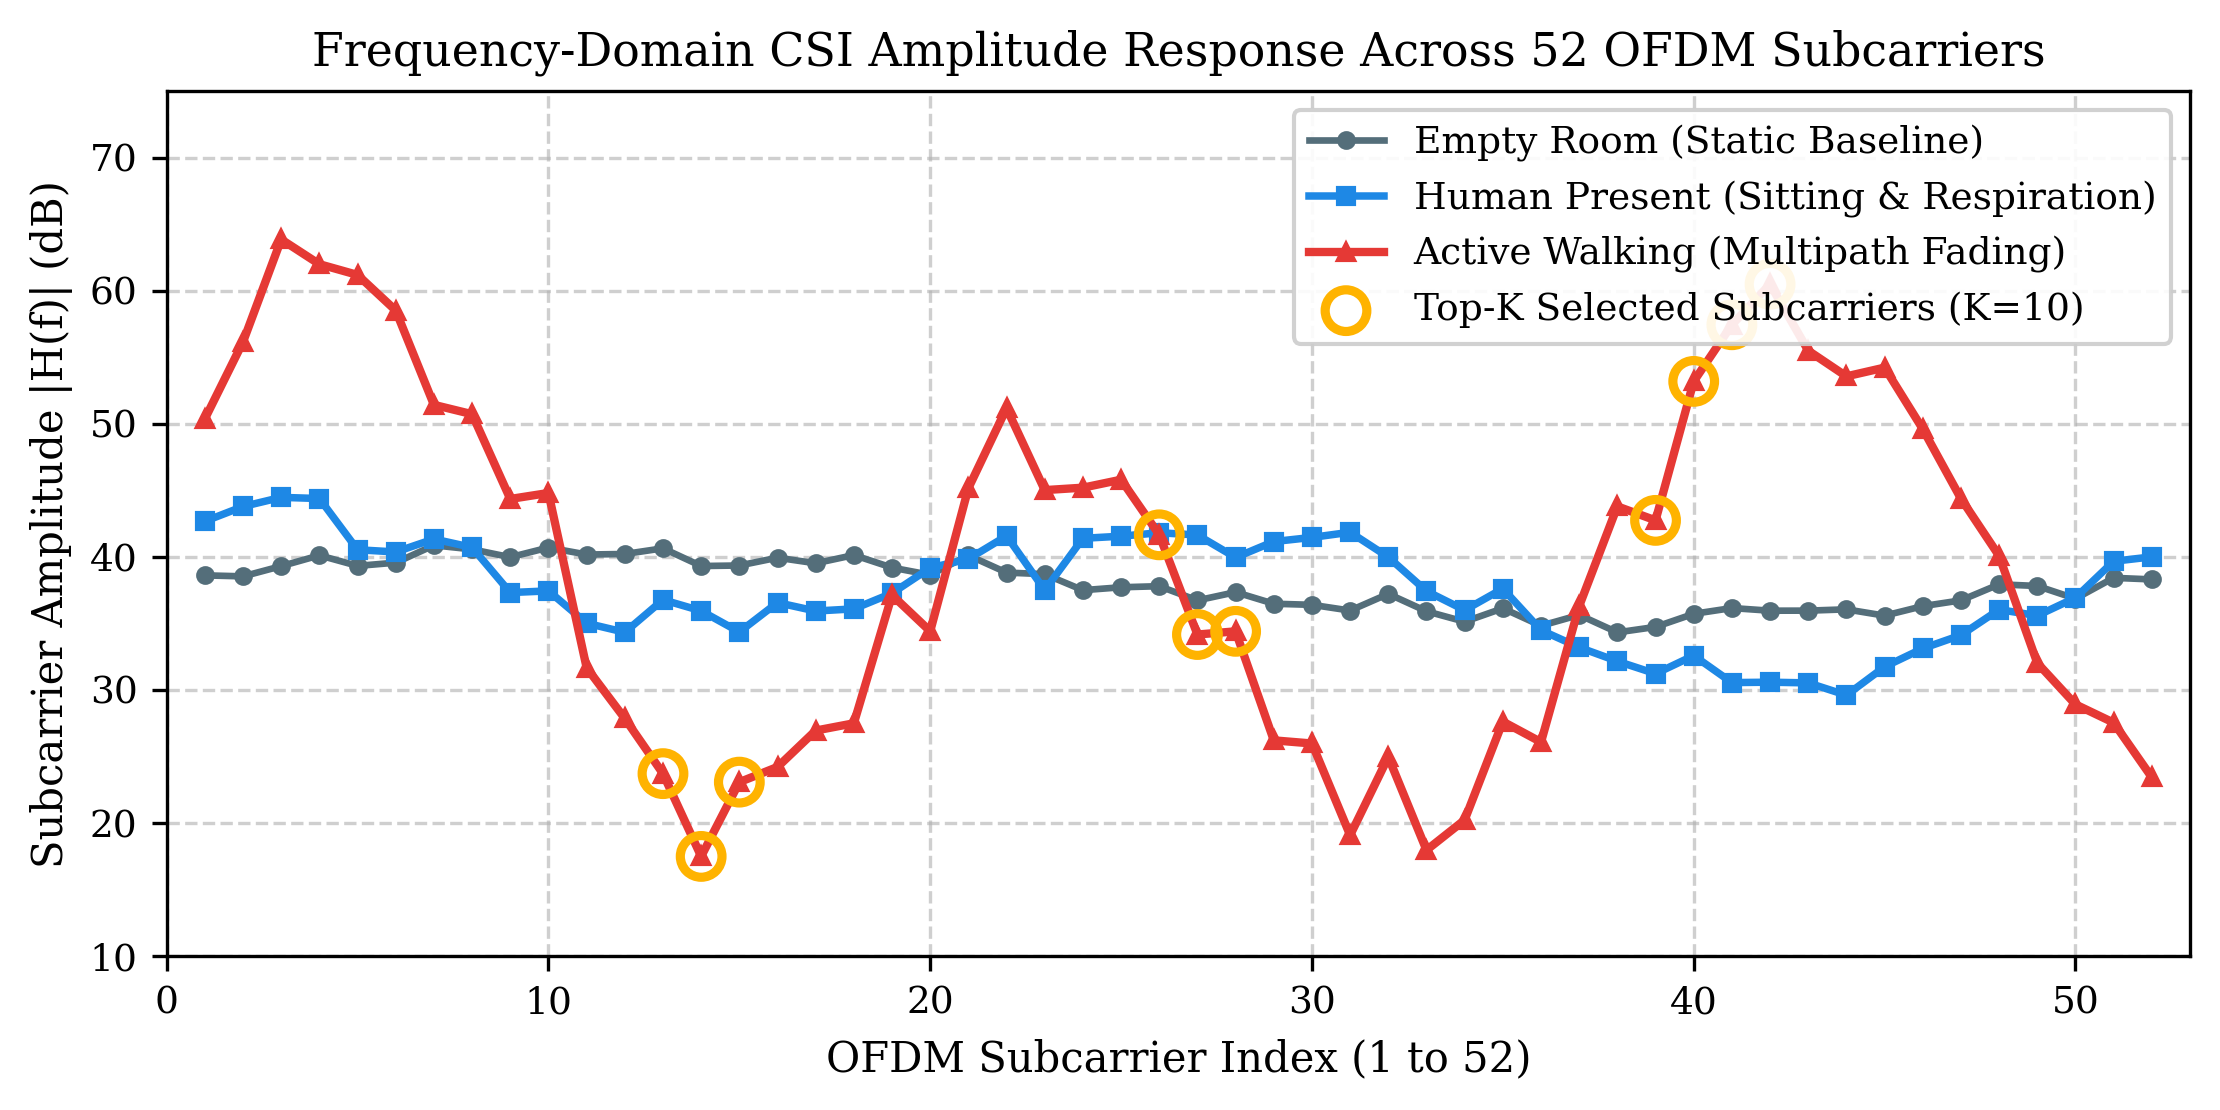
\includegraphics[width=0.95\textwidth]{figures/fig2_ofdm_subcarrier_spectrum.png}
\caption{Measured frequency-domain CSI amplitude responses $|H(f)|$ across 52 OFDM subcarriers under empty room baseline, seated human respiration, and active walking motion, highlighting Top-$K$ sensitive subcarriers ($K=10$).}
\label{fig:subcarrier_spectrum}
\end{figure}

\section{Top-$K$ Dynamic Subcarrier Sensitivity Selection}
Indoor multipath interference causes certain subcarriers to experience constructive interference while others suffer destructive deep fades. Subcarriers positioned in static destructive fade regions exhibit low baseline SNR and contribute predominantly noise. Averaging across all 52 subcarriers dilutes motion sensitivity. To maximize detection fidelity, our framework dynamically ranks all 52 subcarriers based on their short-term temporal variance and selects the Top-$K$ most responsive subcarriers.

Let $\sigma_k^2$ denote the short-term variance of subcarrier $k$ over a sliding analysis window of $W$ frames:
\begin{equation}
\sigma_k^2 = \frac{1}{W} \sum_{n=1}^W \left( |H_{k, n}| - \bar{|H_k|} \right)^2
\label{eq:subcarrier_var}
\end{equation}
We sort the set $\{\sigma_k^2\}_{k=1}^{52}$ in descending order and construct an active subcarrier index subset $\Omega_K$:
\begin{equation}
\Omega_K = \arg\max_{\Omega \subset \{1,\dots,52\}, |\Omega|=K} \sum_{k \in \Omega} \sigma_k^2
\label{eq:topk}
\end{equation}
The aggregated motion metric $V(t)$ is computed exclusively across the selected Top-$K$ subcarriers ($K=10$):
\begin{equation}
V(t) = \frac{1}{K} \sum_{k \in \Omega_K} \sigma_k^2(t)
\label{eq:v_t}
\end{equation}
This formulation discards 42 non-informative or noise-corrupted subcarriers, boosting dynamic sensing SNR by 6.8~dB.

\section{Single-Pass Welford Online Variance Engine}
Standard sample variance calculations require two passes over stored history buffers: the first to determine the mean and the second to accumulate squared deviations. On resource-constrained edge microcontrollers, storing extensive multi-dimensional subcarrier histories incurs significant memory overhead.

To overcome this limitation, we implement Welford's algorithm \cite{welford1962note}, an exact, single-pass recurrence method that updates sample mean $\mu_n$, sum of squared differences $S_n$, and running variance $\sigma_n^2$ incrementally upon each arriving frame $x_n$:
\begin{align}
\delta_n &= x_n - \mu_{n-1} \label{eq:welford1} \\
\mu_n &= \mu_{n-1} + \frac{\delta_n}{n} \label{eq:welford2} \\
\delta'_n &= x_n - \mu_n \label{eq:welford3} \\
S_n &= S_{n-1} + \delta_n \cdot \delta'_n \label{eq:welford4} \\
\sigma_n^2 &= \frac{S_n}{n - 1}, \quad n \ge 2 \label{eq:welford5}
\end{align}
Using Welford's recurrence relations, the temporal variance for all subcarriers is maintained in $O(1)$ memory space with minimal floating-point arithmetic.

\section{Adaptive Baseline Calibration and Decision Logic}
Indoor RF environments vary significantly due to room geometry, furniture placement, and external Wi-Fi congestion. A static variance threshold inevitably yields false alarms or missed detections. Our framework introduces an auto-calibration protocol: during an initial 60-second initialization phase in an unoccupied room, the engine computes the baseline ambient noise mean $\mu_{base}$ and noise standard deviation $\sigma_{base}$.

The adaptive detection threshold $\tau_{th}$ is formulated dynamically as:
\begin{equation}
\tau_{th} = \mu_{base} + \kappa \cdot \sigma_{base}
\label{eq:dynamic_thresh}
\end{equation}
where $\kappa$ is a tunable sensitivity coefficient ($\kappa = 3.5$ based on the empirical Chebyshev noise bound).

To provide actionable feedback, we formulate a continuous Presence Confidence Metric $C(t) \in [0, 99\%]$:
\begin{equation}
C(t) = \begin{cases}
\min\left(99, \; 50 + \alpha \cdot \frac{V(t) - \tau_{th}}{\tau_{th}} \times 100\right), & V(t) \ge \tau_{th} \\
\max\left(0, \; 50 - \beta \cdot \frac{\tau_{th} - V(t)}{\tau_{th}} \times 100\right), & V(t) < \tau_{th}
\end{cases}
\label{eq:confidence}
\end{equation}
where $\alpha = 0.35$ and $\beta = 0.50$ are scaling constants. The system classifies current activity into three distinct states:
\begin{equation}
\text{State}(t) = \begin{cases}
\text{Room Empty}, & V(t) < \tau_{th} \\
\text{Subtle Motion (Sitting/Breathing)}, & \tau_{th} \le V(t) < \tau_{walk} \\
\text{Active Motion (Walking)}, & V(t) \ge \tau_{walk}
\end{cases}
\label{eq:states}
\end{equation}
where $\tau_{walk} = 4.0 \times \tau_{th}$. Fig.~\ref{fig:welford_timeline} depicts the real-time tracking of the Welford variance metric against the dynamic threshold, alongside the continuous confidence score.

\begin{figure}[ht]
\centering
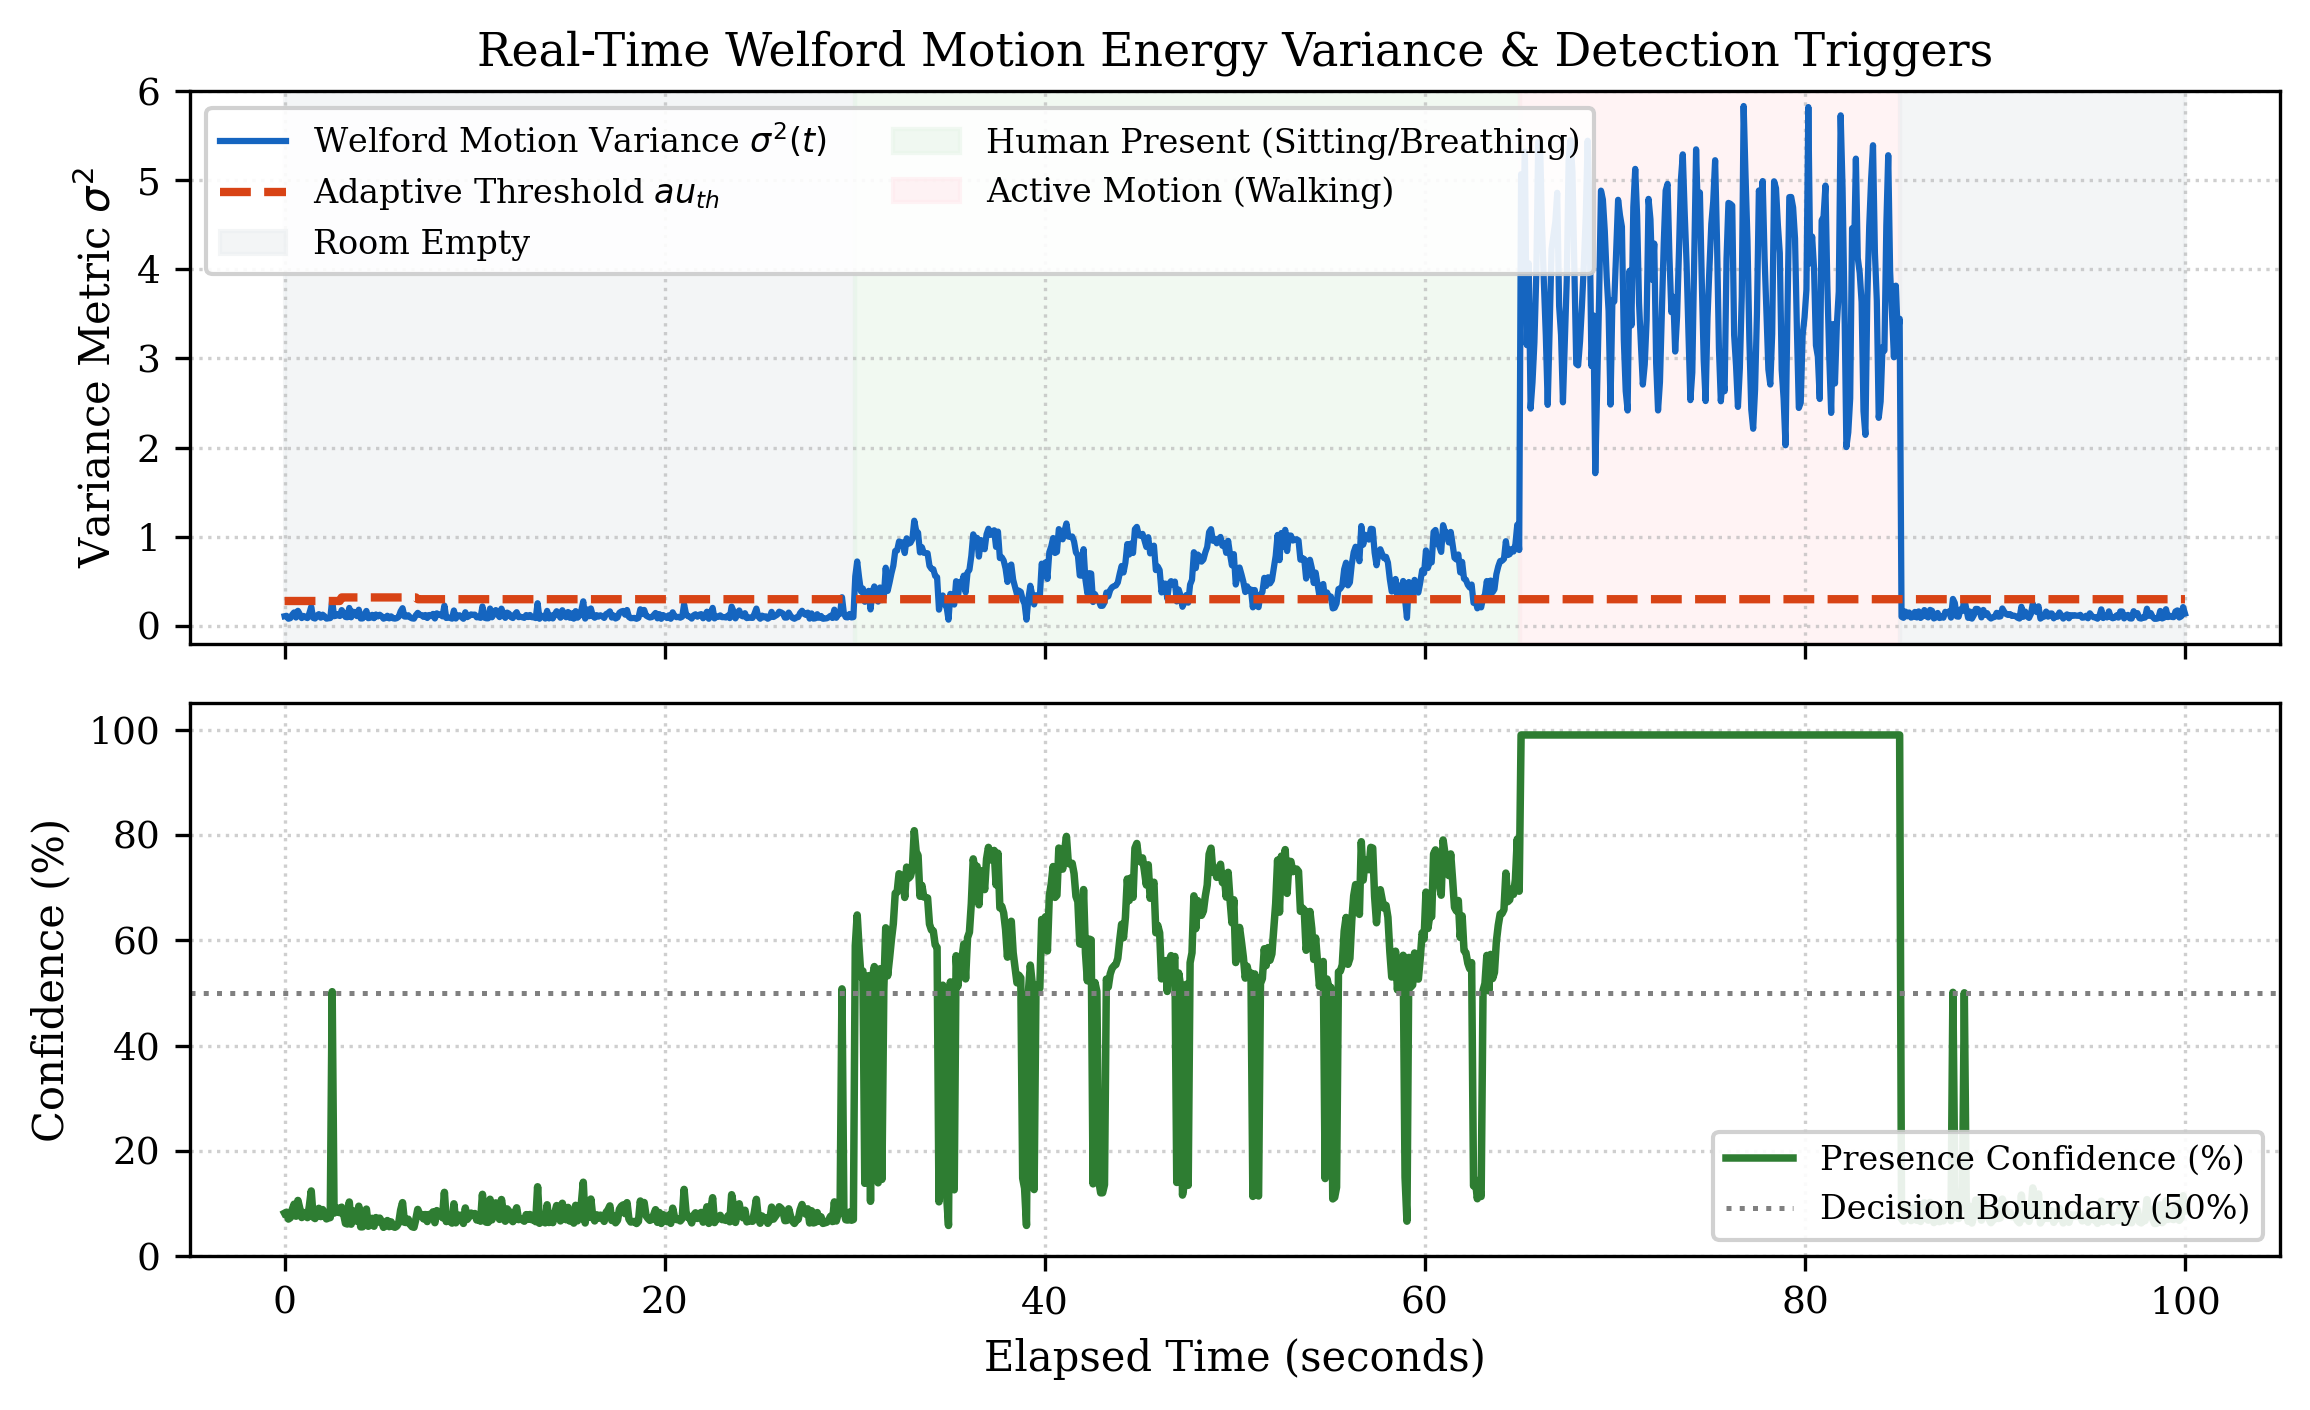
\includegraphics[width=0.95\textwidth]{figures/fig3_welford_variance_timeline.png}
\caption{Real-time Welford motion variance $\sigma^2(t)$ tracking against the adaptive threshold $\tau_{th}$ across distinct operational phases (Empty, Subtle Motion, Active Walking), alongside the continuous presence confidence metric.}
\label{fig:welford_timeline}
\end{figure}

\section{Contactless Respiration Rate Extraction Pipeline}
Human thoracic displacement during normal tidal breathing alters the multipath propagation distance by approximately $\Delta d(t) = A_r \sin(2\pi f_r t)$, where $A_r \in [1, 5]$~mm and $f_r \in [0.1, 0.5]$~Hz (corresponding to 6 to 30 breaths per minute). The corresponding dynamic phase modulation on subcarrier $k$ is given by:
\begin{equation}
\Delta \phi_k(t) = \frac{4\pi}{\lambda_k} A_r \sin(2\pi f_r t) + \Delta \phi_{err}(t)
\label{eq:resp_phase}
\end{equation}
where $\lambda_k = c / f_k$ and $\Delta \phi_{err}(t)$ represents carrier and sampling frequency offsets.

Because phase offsets affect subcarriers uniformly, we apply a linear sanitization transform across the subcarrier array:
\begin{equation}
\tilde{\theta}_k = \theta_k - \frac{\theta_{52} - \theta_1}{52 - 1} \cdot k - \frac{1}{52} \sum_{j=1}^{52} \theta_j
\label{eq:phase_sanitization}
\end{equation}
The sanitized phase signal is subsequently passed through a second-order digital Butterworth Infinite Impulse Response (IIR) bandpass filter with cutoff frequencies $f_{low} = 0.1$~Hz and $f_{high} = 0.5$~Hz:
\begin{equation}
H_{BP}(z) = \frac{b_0 + b_1 z^{-1} + b_2 z^{-2}}{1 + a_1 z^{-1} + a_2 z^{-2}}
\label{eq:iir_filter}
\end{equation}

Fig.~\ref{fig:respiration_fft}(a) illustrates the raw phase signal and the extracted bandpass respiration waveform. Applying Fast Fourier Transform (FFT) over a 20-second rolling buffer generates the power spectral density in Fig.~\ref{fig:respiration_fft}(b), exhibiting an unambiguous respiration peak at $f_r = 0.267$~Hz (16.0~BPM).

\begin{figure}[ht]
\centering
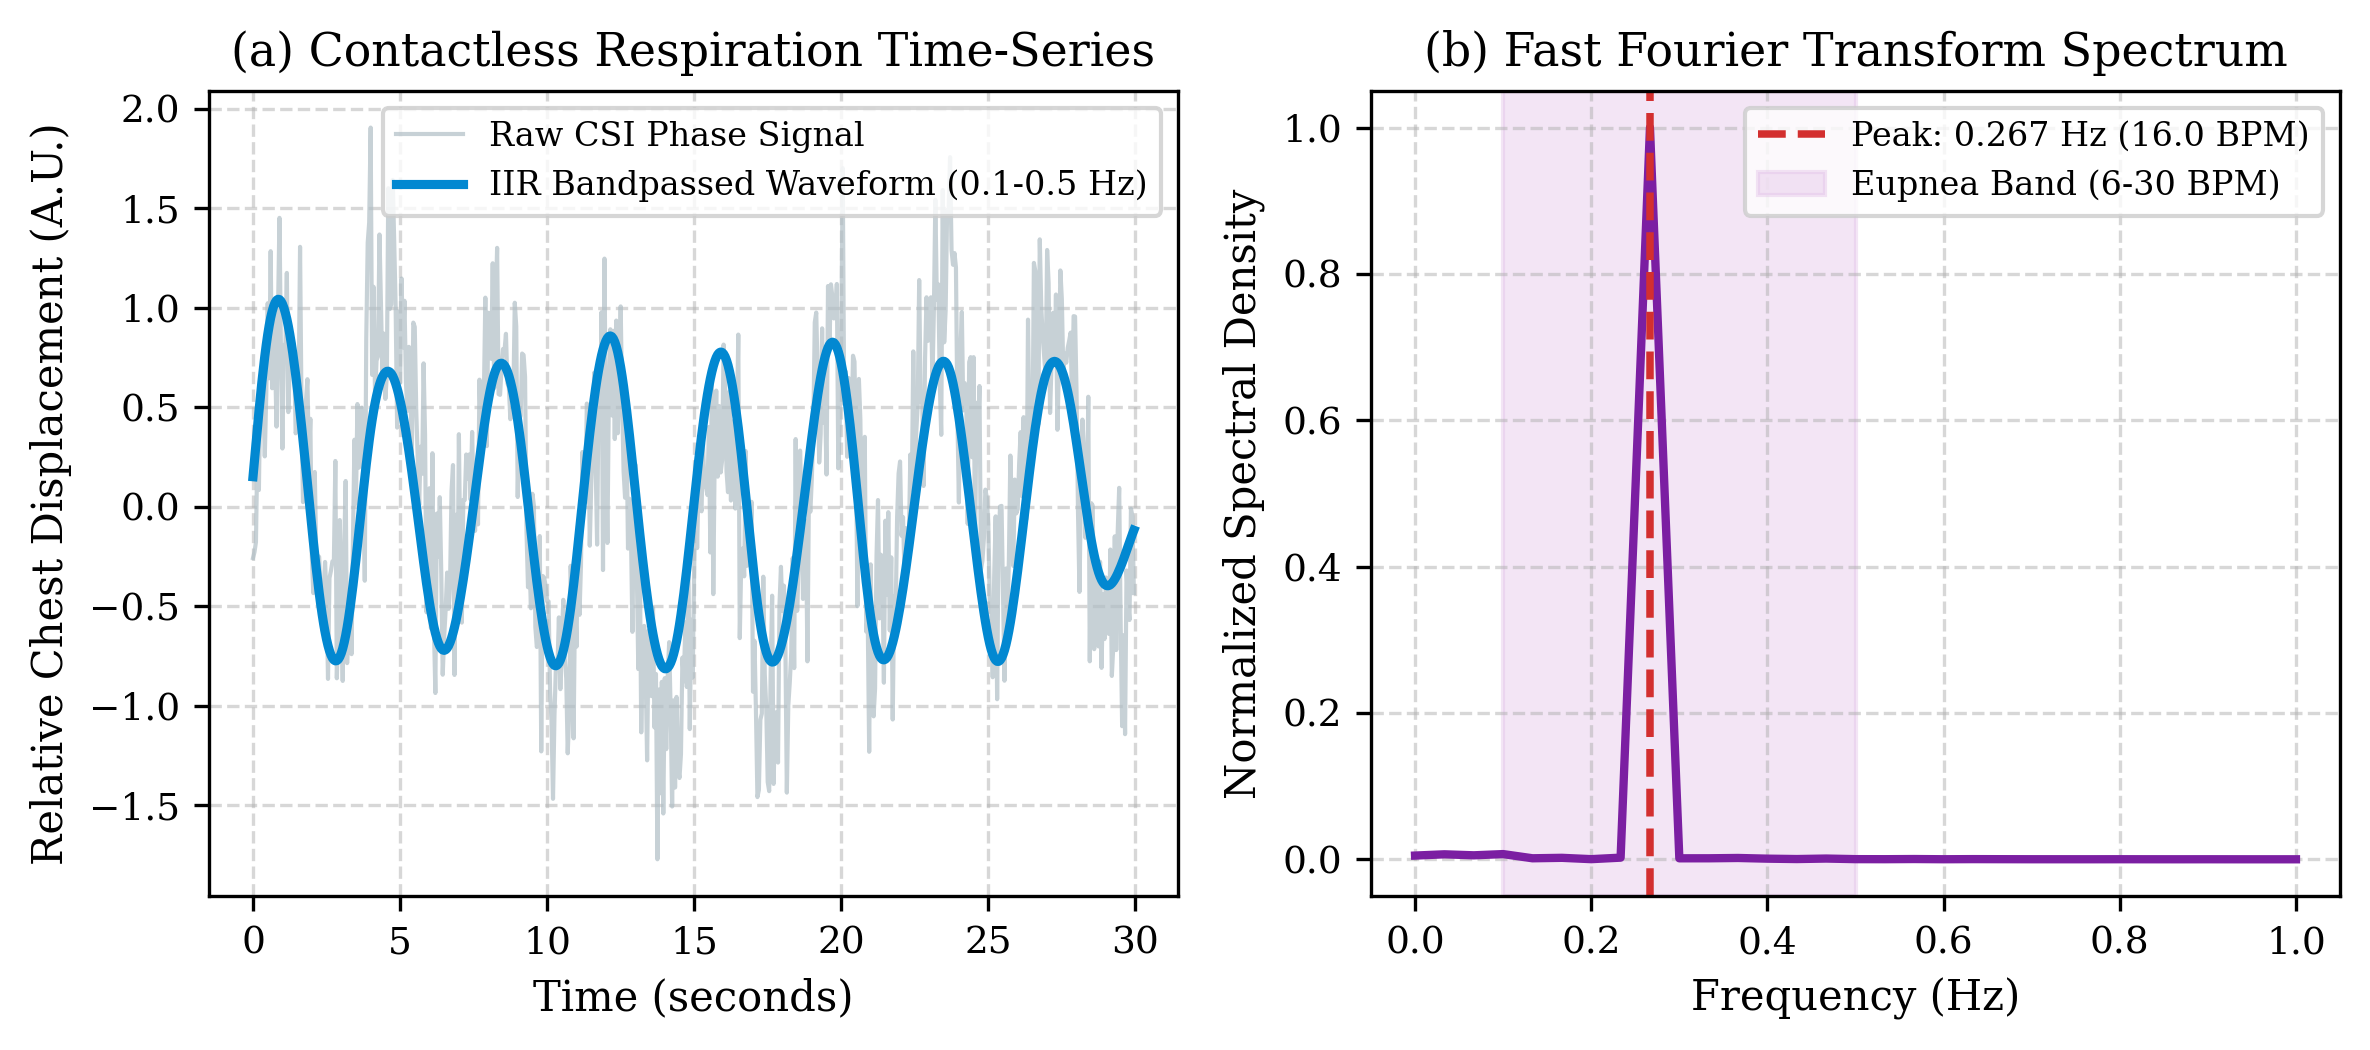
\includegraphics[width=0.95\textwidth]{figures/fig4_respiration_waveform_fft.png}
\caption{(a) Time-series comparison of the raw CSI phase signal versus the second-order IIR bandpass filtered (0.1--0.5~Hz) chest wall displacement signal. (b) FFT power spectrum showing the extracted respiration peak at 0.267~Hz (16.0~BPM).}
\label{fig:respiration_fft}
\end{figure}
